\subsection{Robustness of the Empirical Association}\label{sec:robustness}
To ensure that the observed association between multi-PR status and closure delay is not an artifact of specific filtering choices, we executed seven pre-planned sensitivity tests (Table~\ref{tab:robustness} and Fig.~\ref{fig:robustness}):
\begin{itemize}
  \item \textbf{R1 (Broad bug labels)}: Expanding classification to include symptom labels (e.g., \texttt{crash}, \texttt{regression}).
  \item \textbf{R2 (Unfiltered link tuples)}: Grouping on raw unresolved link references (identical to baseline, as all cohort links resolve).
  \item \textbf{R3 (Merged PR requirement)}: Restricting to issues where at least one linked PR was merged into the main branch.
  \item \textbf{R4 (Continuous PR count)}: Evaluating rank correlation across all $k \ge 1$.
  \item \textbf{R5 (High-volume projects)}: Restricting to repositories containing at least 5 issues in both Group A and Group B.
  \item \textbf{R6 (Duration truncation)}: Truncating extreme outliers ($>3{,}000$ days) and excluding sub-hour triage tickets ($<1$ hour).
  \item \textbf{R7 (Dominant project removal)}: Dropping the single largest contributing repository from each group.
\end{itemize}

\begin{table}[t]
\centering
\caption{Robustness checks R1--R7 for the primary comparison (all tests Mann--Whitney $U$ unless noted).\label{tab:robustness}}
\small \resizebox{\textwidth}{!}{%
\begin{tabular}{@{}lrrrrrccc@{}}
\toprule
Check & $n_A$ & $n_B$ & Med.\ A & Med.\ B & Diff & $p$ & Cliff's $\delta$ & Same dir.? \\\midrule
Baseline (strict label, matched links) & 14,280 & 662 & 8.0 & 35.3 & 27.3 & $3.31\times 10^{-35}$ & 0.284 & yes \\
R1 broader bug definition & 17,590 & 797 & 6.6 & 32.3 & 25.7 & $7.85\times 10^{-51}$ & 0.314 & yes \\
R2 group on all link references & 14,280 & 662 & 8.0 & 35.3 & 27.3 & $3.31\times 10^{-35}$ & 0.284 & yes \\
R3 at least one merged linked PR & 13,877 & 639 & 7.8 & 33.7 & 25.8 & $1.14\times 10^{-33}$ & 0.283 & yes \\
R4 PR count continuous (Spearman) & \multicolumn{4}{l}{14,942 issues with $\geq 1$ link} & Spearman $\rho$=0.101 & $1.72\times 10^{-35}$ & -- & yes \\
R5 projects with $\geq$5 per group & 10,026 & 522 & 7.4 & 33.2 & 25.8 & $5.15\times 10^{-30}$ & 0.295 & yes \\
R6 winsorised at 180 days & 14,280 & 662 & 8.0 & 35.3 & 27.3 & $7.34\times 10^{-35}$ & 0.282 & yes \\
R6 winsorised at 365 days & 14,280 & 662 & 8.0 & 35.3 & 27.3 & $2.75\times 10^{-35}$ & 0.284 & yes \\
R6b drop durations $<$1 hour & 13,942 & 656 & 8.7 & 35.9 & 27.3 & $1.28\times 10^{-33}$ & 0.279 & yes \\
R7 drop largest project per group & 13,058 & 606 & 7.9 & 38.8 & 30.9 & $2.02\times 10^{-37}$ & 0.307 & yes \\
\bottomrule
\end{tabular}
}
\par\vspace{2pt}{\footnotesize\textit{Note: R2 is identical to the baseline by construction:}}
\par\vspace{2pt}{\footnotesize\textit{Note: the cohort contains zero unmatched link references.}}
\end{table}


\begin{figure}[htbp]\centering
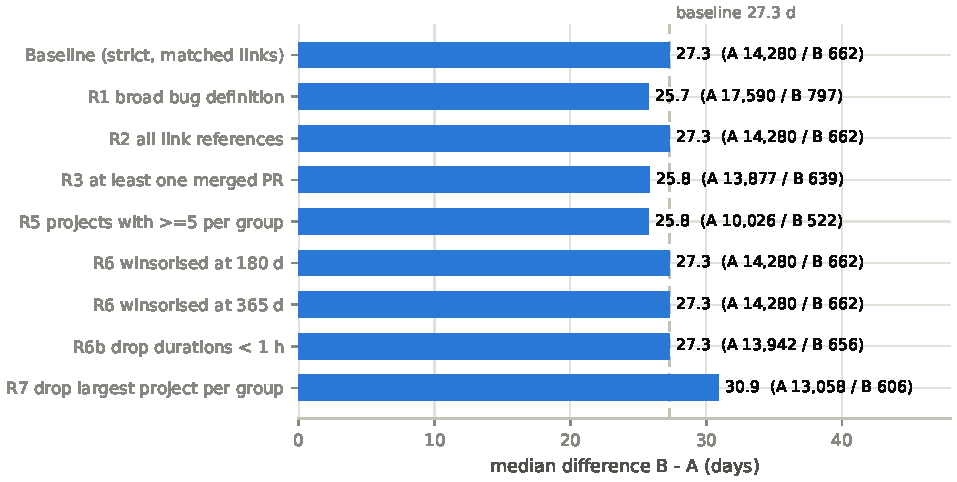
\includegraphics[width=.62\linewidth]{figures/fig6_robustness.pdf}
\caption{Robustness checks R1--R7: median differences (days) and Cliff's $\delta$ effect sizes.\label{fig:robustness}}
\end{figure}

The empirical direction holds across all seven checks: Cliff's $\delta$ remains confined within a narrow band (0.279 to 0.314, all $p < 10^{-10}$), confirming that the raw statistical association is robust.

\subsection{The Fixed-Landmark Finding: Disentangling Link Accumulation}\label{sec:landmark}
The core inquiry is whether the raw \valmedDiff-day gap reflects genuine resolution friction or reverse-causality link accumulation.

\textbf{Exposure-Restricted Subset.} Restricting the analysis to issues whose linked PRs were all created within the initial 50\% of the issue's lifespan reduces the median gap from \valmedDiff{}~days to \valdetDiff{}~days (Group B median \valdetMedB{} vs.\ Group A \valdetMedA{}~days; $n_A=\valdetNA$, $n_B=\valdetNB$; $\delta = \valdetD$, $p = \valdetP$). However, because selecting this subset conditions on the final closure date (the outcome itself), it acts as an informative upper bound rather than an unbiased causal estimate.

\textbf{Fixed-Landmark Analysis (Primary $L=30$ days).} Among the \vallmCohort{} issues in Groups A and B, \vallmClosed{} issues closed prior to day~30 and drop out of the at-risk set. Among the remaining \vallmAtRisk{} open issues at day~30, their landmark status was:
\begin{itemize}
  \item \vallmNZero{} issues had accumulated \textbf{zero} linked PRs by day~30.
  \item \vallmNOne{} issues had accumulated \textbf{exactly one} linked PR by day~30.
  \item Only \vallmNM{} issues had accumulated \textbf{two or more} linked PRs by day~30.
\end{itemize}

When we measure the subsequent calendar duration from day~30 until closure, the gap between one-PR and multi-PR issues \textbf{completely vanishes}:
\begin{equation}
\text{Median}(\ge 2\text{ PRs}) - \text{Median}(1\text{ PR}) = \vallmMedM{} - \vallmMedOne{} = \vallmDiff\text{ days}
\end{equation}
The difference is statistically indistinguishable from zero ($\delta = \vallmD$, $p = \vallmP$, Mann--Whitney $U$). The project-clustered 95\% confidence interval spans \vallmCI{}~days, firmly straddling zero (Table~\ref{tab:landmark}). Within individual repositories, among the \vallmSignN{} projects with both landmark groups at day~30, multi-PR issues close slower in \vallmSignW{} projects and faster in 9 ($p=\vallmSignP$---equivalent to a random coin toss).

\begin{table}[t]
\centering
\caption{Fixed-landmark analysis: among issues still open $L$ days after creation, additional days from the landmark to closure, by number of linked PRs created by day $L$ (Mann--Whitney $U$; project-clustered bootstrap CI).\label{tab:landmark}}
\small \resizebox{\textwidth}{!}{%
\begin{tabular}{@{}lrrrrrrrrrrc@{}}
\toprule
Landmark & Still open & Closed before & $n_0$ & $n_1$ & $n_{\geq 2}$ & Med.\ 1-PR & Med.\ $\geq$2-PR & Diff. & $\delta$ & $p$ & 95\% CI (days) \\\midrule
7 d & 7,928 & 7,014 & 6225 & 1656 & 47 & 8.3 & 3.2 & -5.1 & -0.207 & $0.0154$ & [-6.8, -1.4] \\
30 d & 4,909 & 10,033 & 4063 & 813 & 33 & 30.0 & 29.2 & -0.8 & -0.022 & $0.832$ & [-22.5, 29.2] \\
90 d & 3,094 & 11,848 & 2623 & 449 & 22 & 66.3 & 87.5 & 21.2 & 0.059 & $0.641$ & [-41.3, 189.0] \\
\bottomrule
\end{tabular}
}
\par\vspace{2pt}{\footnotesize\textit{Note: $n_0/n_1/n_{\geq 2}$: issues with 0, 1, $\geq$2 linked PRs created by day $L$; the comparison column pair uses only the 1-PR and $\geq$2-PR groups.}}
\end{table}


Two decisive mechanisms account for this finding:
\begin{enumerate}
  \item \textbf{Late Link Assembly}: \textbf{\vallmShareB{}} of original Group-B issues had not yet accumulated two PRs by day~30. Their multi-PR status was assembled in the second half of an already-prolonged open lifecycle.
  \item \textbf{The True Bottleneck is Zero PR Activity}: Issues with \emph{no} linked PR by day~30 suffered severe subsequent delays, requiring a median of \vallmMedZ{} additional days to close after the landmark, compared to only \vallmMedM{} days for the multi-PR cohort ($\delta = \vallmZD$, $p = \vallmZP$).
\end{enumerate}

\textbf{Sensitivity at $L=7$ and $L=90$ days.} At an early landmark of $L=7$ days, multi-PR issues ($n=47$ at risk) closed 5.1 days \emph{faster} ($p=0.015$), indicating that early multi-PR activity reflects intense, active contributor focus. At $L=90$ days, the subsequent difference is small and statistically non-significant ($+21.2$ days, 95\% CI $-41.3$ to $+189.0$ days, $n=22$ multi-PR). 

In summary, once the link-accumulation channel is controlled, having multiple linked PRs does not cause substantive resolution delays. The raw 27.3-day delay is predominantly an artifact of open issues accumulating pull requests over time.
